\subsection{Hyperparameter Tuning}\label{hyperparameter-tuning}

\begin{table}[th]
    \captionsetup{aboveskip=\tableaboveskip,belowskip=\tablebelowskip}
    \caption{\textbf{Reference vs Optimal $(\alpha, \Delta T)$ on CIFAR-10.} Optimal hyperparameters are obtained by tuning with a TPE sampler in Optuna. The difference between the reference and optimal performance is small, indicating that there is not a significant benefit in tuning $(\alpha, \Delta T)$ individually for each initialization and sparsity configuration.}
    \label{tab:effect-alpha-deltaT}
    \centering
    
    \begin{tabular}{ c c  cc  cc}
    \toprule
    \multirow{3}{*}{\textbf{Initialization}} & \textbf{Density} & 
    \multicolumn{2}{c}{\textbf{Reference}} & \multicolumn{2}{c}{\textbf{Optimal}} \\
    \cmidrule(lr){2-2} \cmidrule(lr){3-4} \cmidrule(lr){5-6}
    {} & {$(1-s)$} & 
    {$(\alpha, \Delta T)$} & \makecell{Accuracy $\uparrow$ \\ (Test)} & 
    {$(\alpha, \Delta T)$} & \makecell{Accuracy $\uparrow$ \\ (Test)} \\
    \midrule
    
    Random & 0.1 & 
    {0.3, 100} & {91.7 $\pm$ 0.18} &  
    {0.197, 50} & \textbf{91.8 $\pm$ 0.17} \\
    
    Random & 0.2 & 
    {0.3, 100} & {92.6 $\pm$ 0.10} &  
    {0.448, 150} & \textbf{92.8 $\pm$ 0.16} \\
    
    Random & 0.5 & 
    {0.3, 100} & \textbf{93.3 $\pm$ 0.07} &  
    {0.459, 550} & \textbf{93.3 $\pm$ 0.18} \\
    \midrule
    
    ERK & 0.1 & 
    {0.3, 100} & \textbf{92.4 $\pm$ 0.06} &  
    {0.416, 200} & \textbf{92.4 $\pm$ 0.23} \\
    
    ERK & 0.2 & 
    {0.3, 100} & \textbf{93.1 $\pm$ 0.09} &  
    {0.381, 950} & \textbf{93.1 $\pm$ 0.21} \\
    
    ERK & 0.5 & 
    {0.3, 100} & {93.4 $\pm$ 0.14} &  
    {0.287, 500} & \textbf{93.8 $\pm$ 0.06} \\
    \hline

    \end{tabular}
    
    \label{tab:replication_verify}
\end{table}

\subsubsection{$(\alpha, \Delta T)$ vs Sparsities} To understand the impact of the two additional hyperparameters included in \textit{RigL}, we use a Tree of Parzen Estimator (TPE sampler, \citet{TPE_Bergstra}) via Optuna to tune $(\alpha, \Delta T)$. We do this for sparsities $(1 - s) \in \{0.1,0.2,0.5\}$, and a fixed learning rate of $0.1$. Additionally, we set the sampling domain for $\alpha$ and $\Delta T$ as $[0.1,0.6]$ and $\{50,100, 150,...,1000\}$ respectively. We use 15 trials for each sparsity value, with our objective function as the validation accuracy averaged across 3 random seeds.\\

\begin{figure}[!b]
    \centering
    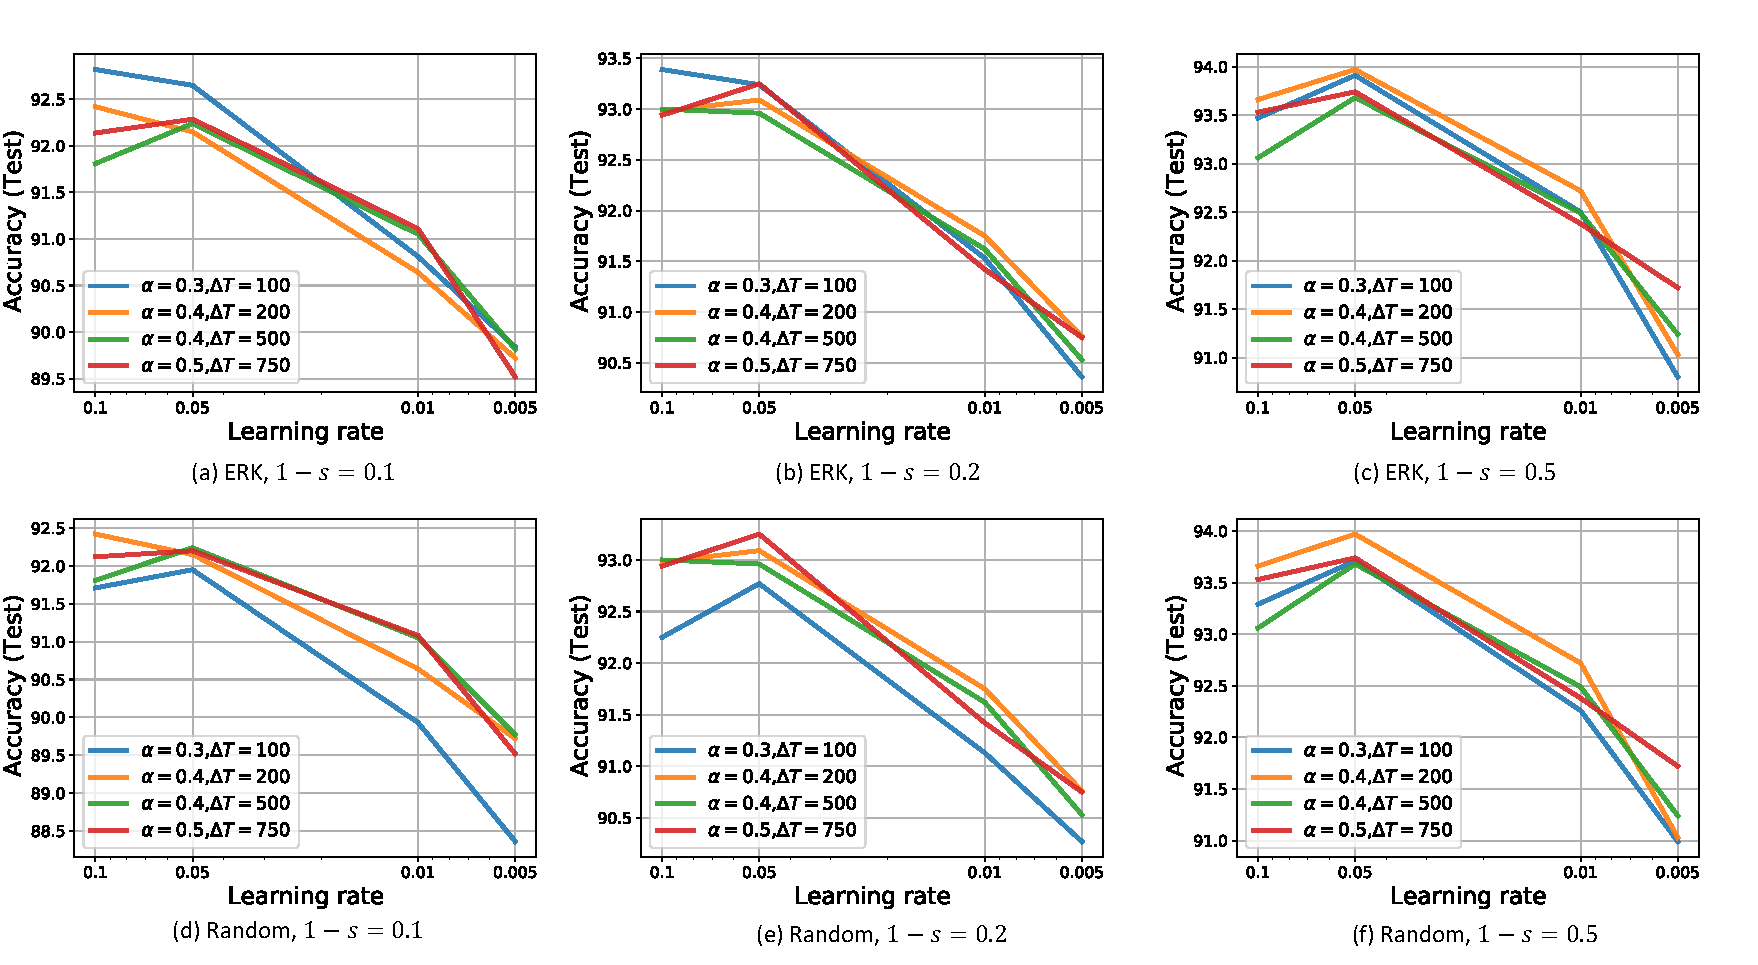
\includegraphics[width=\textwidth]{../openreview/figs/lr_sweep.pdf}
    \captionsetup{aboveskip=\figureaboveskip,belowskip=\figurebelowskip}
    \caption{\textbf{Learning Rate vs Sparsity on CIFAR-10.} Runs using a learning rate $> 0.1$ do not converge and are not plotted here. There is little benefit in tuning the learning rate for each sparsity, and $0.1, 0.05$ are good choices overall.}
    \label{fig:lr-sweep}
\end{figure}

Table \ref{tab:effect-alpha-deltaT} shows the test accuracies of tuned hyperparameters. While the reference hyperparameters (original authors, $\alpha=0.3, \Delta T=100$) differ from the obtained optimal hyperparameters, the difference in performance is marginal, especially for ERK initialization. This in agreement with the original paper, which finds $\alpha \in \{0.3, 0.5\}, \Delta T = 100$ to be suitable choices. We include contour plots detailing the hyperparameter trial space in the supplementary material.

\subsubsection{Learning Rate vs Sparsities} We further examine if the final performance improves by tuning the learning rate ($\eta$) individually for each sparsity-initialization pair. We employ a grid search over $\eta \in $ \{$0.1,0.05,0.01,0.005$\} and $(\alpha, \Delta T) \in$ \{$(0.3, 100)$, $(0.4,200)$, $(0.4, 500)$, $(0.5, 750)$\}. As seen in Figure \ref{fig:lr-sweep}, $\eta = 0.1$ and $\eta = 0.05$ are close to optimal values for a wide range of sparsities and initializations. Since these learning rates also correspond to good choices for the Dense baseline, one can employ similar values when training with \textit{RigL}.

